\section{Wstęp}
\label{sec:wstep}

Celem pracy jest numeryczne wyznaczenie optymalnego sterowania dla zadania sterowania elektryczną deskorolką lub pojazdem typu \textit{Segway}. Składają się one z platformy i dwóch kół umieszczonych z boków. Pasażer stoi na platformie. Temat uznano za szczególnie ciekawy ze względu na stale rosnącą popularność Segwayów. Pierwszy tego typu pojazd został komercyjnie sprzedany w 2002 roku za kwotę 100 tys. amerykańskich dolarów! Dzisiaj użytkowników Segwayów możemy zobaczyć praktycznie wszędzie, zaczynając od pracowników supermarketów, a kończąc na turystach sprawnie poruszających się po najbardziej zatłoczonych ulicach miasta. Jego ogromną zaletą jest możliwość poruszania na zewnątrz, jak również wewnątrz większych budynków i hal. Obecnie trwają prace nad przystosowaniem Segwaya do transportu ludzi niepełnosprawnych. Brano pod uwagę również możliwość zdalnego transportu obiektu za pomocą tego urządzenia. W tym wypadku zamiast pasażera na platformie znajdowałby się ładunek. Efektem sterowania ma być przesunięcie urządzenia do zadanego punktu w przestrzeni jednowymiarowej (początkowo zakłada się ruch w przód i w tył) oraz dwuwymiarowej (koła mają różną prędkość obrotową). Jego położenie kątowe stabilizowane jest w niestabilnym punkcie równowagi (pionowo w górę). Trudności w sterowaniu są spowodowane nieliniowością dynamiki obiektu. Kryterium do oceny stanowić może zużycie energii, czas potrzebny do osiągnięcia pozycji lub dokładność osiągniętej pozycji po zadanym czasie. %Zaproponowane sterowanie postanowiono porównać z klasycznym podejściem, wykorzystującym regulator typu PID.

\begin{figure}[h]
	\centering
	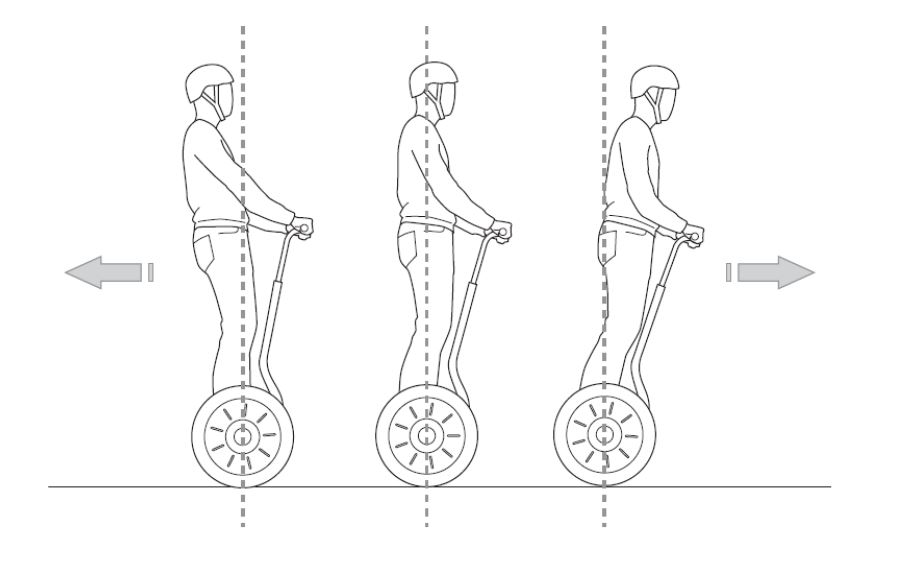
\includegraphics[width=4in]{Figures/wstep_segway.jpg}
	\captionsource{Działanie pojazdu \textit{Segway}.}{\cite{Babazadeh}}
	\label{fig:wstep_segway}
\end{figure}

Zadanie to wymaga wyznaczenia modelu matematycznego badanego obiektu oraz przetestowania jego działania. Następnie, na podstawie modelu, należy wyznaczyć optymalne sterowanie.